% Q1V1: E-core with Center-Limb Air Gap — Exam diagram (hybrid style C)
% Shows: core geometry, coil positions, gap location, dimensions
% Strips: flux arrows, mu_r label, reluctance circuit (P-STACK-31)
\documentclass[border=10pt]{standalone}
\usepackage{tikz}
\usepackage{amsmath}
\usetikzlibrary{patterns, decorations.pathreplacing}
\renewcommand{\familydefault}{\sfdefault}

\begin{document}
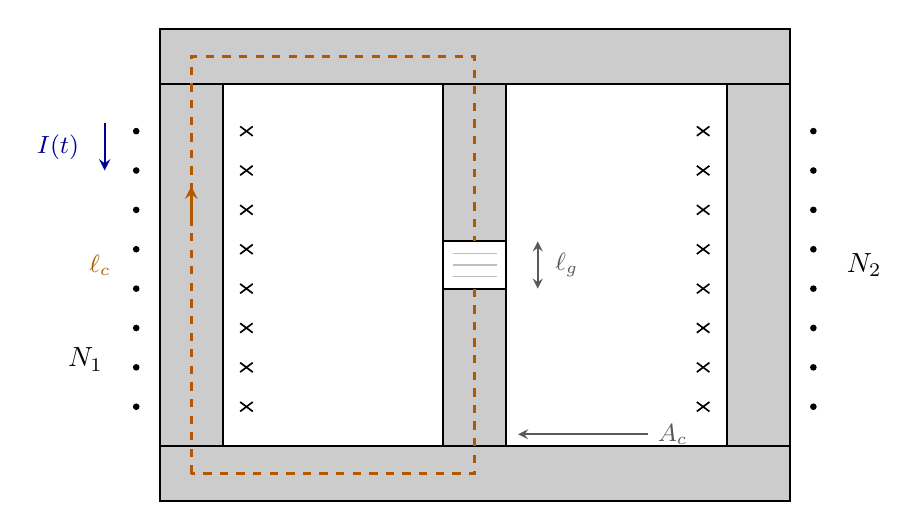
\begin{tikzpicture}[
    every node/.style={font=\sffamily},
    >=stealth,
    dim/.style={<->, line width=0.6pt, gray!70!black},
    dimlabel/.style={font=\sffamily\small, text=gray!70!black},
]

% === Core dimensions ===
\def\coreW{8}       % total width
\def\coreH{6}       % total height (bottom bar to top bar top)
\def\barH{0.7}      % yoke (horizontal bar) height
\def\limbW{0.8}     % limb width
\def\gapH{0.6}      % air gap height

% === E-piece (bottom yoke + three limbs) ===
% Bottom yoke
\fill[gray!40, draw=black, line width=0.8pt]
    (0,0) rectangle (\coreW,\barH);

% Left limb
\fill[gray!40, draw=black, line width=0.8pt]
    (0,\barH) rectangle (\limbW,{\coreH-\barH});

% Center limb (below gap)
\fill[gray!40, draw=black, line width=0.8pt]
    ({0.5*\coreW-0.5*\limbW},\barH) rectangle ({0.5*\coreW+0.5*\limbW},{0.5*\coreH-0.5*\gapH});

% Right limb
\fill[gray!40, draw=black, line width=0.8pt]
    ({\coreW-\limbW},\barH) rectangle (\coreW,{\coreH-\barH});

% === I-piece (top yoke + center limb above gap) ===
% Top yoke
\fill[gray!40, draw=black, line width=0.8pt]
    (0,{\coreH-\barH}) rectangle (\coreW,\coreH);

% Center limb (above gap)
\fill[gray!40, draw=black, line width=0.8pt]
    ({0.5*\coreW-0.5*\limbW},{0.5*\coreH+0.5*\gapH}) rectangle ({0.5*\coreW+0.5*\limbW},{\coreH-\barH});

% === Air gap (hatched) ===
\fill[white]
    ({0.5*\coreW-0.5*\limbW},{0.5*\coreH-0.5*\gapH})
    rectangle ({0.5*\coreW+0.5*\limbW},{0.5*\coreH+0.5*\gapH});
\draw[line width=0.8pt]
    ({0.5*\coreW-0.5*\limbW},{0.5*\coreH-0.5*\gapH})
    rectangle ({0.5*\coreW+0.5*\limbW},{0.5*\coreH+0.5*\gapH});
% Hatching inside gap
\foreach \yy in {0.15, 0.30, 0.45} {
    \draw[thin, gray!50]
        ({0.5*\coreW-0.35*\limbW},{0.5*\coreH-0.5*\gapH+\yy})
        -- ({0.5*\coreW+0.35*\limbW},{0.5*\coreH-0.5*\gapH+\yy});
}

% === Coil 1 (left limb) ===
\foreach \ycoil in {1.2, 1.7, 2.2, 2.7, 3.2, 3.7, 4.2, 4.7} {
    % Outer winding mark (dot = out of page)
    \fill ({-0.3},\ycoil) circle (1.2pt);
    % Inner winding mark (cross = into page)
    \draw[line width=0.6pt] ({\limbW+0.22},{\ycoil-0.06}) -- ({\limbW+0.38},{\ycoil+0.06});
    \draw[line width=0.6pt] ({\limbW+0.22},{\ycoil+0.06}) -- ({\limbW+0.38},{\ycoil-0.06});
}
\node[left, font=\sffamily] at (-0.6, 1.8) {$N_1$};

% === Coil 2 (right limb) ===
\foreach \ycoil in {1.2, 1.7, 2.2, 2.7, 3.2, 3.7, 4.2, 4.7} {
    % Inner winding mark (cross = into page)
    \pgfmathsetmacro{\innerX}{\coreW-\limbW-0.3}
    \draw[line width=0.6pt] ({\innerX-0.08},{\ycoil-0.06}) -- ({\innerX+0.08},{\ycoil+0.06});
    \draw[line width=0.6pt] ({\innerX-0.08},{\ycoil+0.06}) -- ({\innerX+0.08},{\ycoil-0.06});
    % Outer winding mark (dot = out of page)
    \fill ({\coreW+0.3},\ycoil) circle (1.2pt);
}
\node[right, font=\sffamily] at ({\coreW+0.6}, 3.0) {$N_2$};

% === Dimension: air gap length ===
\draw[dim] ({0.5*\coreW+0.5*\limbW+0.4},{0.5*\coreH-0.5*\gapH})
        -- ({0.5*\coreW+0.5*\limbW+0.4},{0.5*\coreH+0.5*\gapH});
\node[dimlabel, right] at ({0.5*\coreW+0.5*\limbW+0.5},{0.5*\coreH}) {$\ell_g$};

% === Dimension: cross-sectional area ===
\draw[->, line width=0.6pt, gray!70!black]
    ({0.5*\coreW+0.5*\limbW+1.8},{0.5*\barH+0.5})
    -- ({0.5*\coreW+0.5*\limbW+0.15},{0.5*\barH+0.5});
\node[dimlabel, right] at ({0.5*\coreW+0.5*\limbW+1.8},{0.5*\barH+0.5}) {$A_c$};

% === Mean magnetic path (dashed centerline through core) ===
% Left window: left limb center → top yoke center → center limb center → bottom yoke center
\draw[dashed, line width=1.0pt, orange!70!black]
    ({0.5*\limbW},{0.5*\barH})                          % bottom-left corner
    -- ({0.5*\limbW},{\coreH-0.5*\barH})                % up left limb
    -- ({0.5*\coreW},{\coreH-0.5*\barH})                % right along top yoke
    -- ({0.5*\coreW},{0.5*\coreH+0.5*\gapH})            % down center limb (to gap top)
    ({0.5*\coreW},{0.5*\coreH-0.5*\gapH})               % resume below gap
    -- ({0.5*\coreW},{0.5*\barH})                        % down to bottom yoke
    -- ({0.5*\limbW},{0.5*\barH});                       % left along bottom yoke
\node[dimlabel, left, text=orange!70!black] at (-0.5, {0.5*\coreH}) {$\ell_c$};
% Arrow indicator on the path
\draw[->, orange!70!black, line width=1.0pt] ({0.5*\limbW},{3.5}) -- ({0.5*\limbW},{4.0});

% === Current arrow on primary ===
\draw[->, thick, blue!60!black] (-0.7, 4.8) -- (-0.7, 4.2);
\node[left, font=\sffamily\small, text=blue!60!black] at (-0.9, 4.5) {$I(t)$};

\end{tikzpicture}
\end{document}
